\documentclass[12pt, a4paper]{article}
\usepackage[dvips, bottom=2.5cm, top=2.5cm, right=2.5cm, left=3cm]{geometry}
\usepackage[utf8]{inputenc}
\usepackage[ngerman]{babel}
\usepackage[babel,german=quotes]{csquotes}
\usepackage[T1]{fontenc}
\usepackage{enumerate}
\usepackage{setspace}
\usepackage{mdframed}
\setstretch{1.3} 
\setlength\parindent{0pt}
\usepackage{textcomp}
\usepackage{enumerate}
\usepackage{color}
\usepackage{graphicx}
\usepackage{colortbl}
\usepackage{hhline}
\usepackage{tabularx}
\usepackage{booktabs}
\usepackage[font={footnotesize}, labelfont=bf]{caption}
\usepackage[dvipsnames]{xcolor}
\usepackage{float}
\usepackage{subfig}

%: ================================
%: Anfang
%: ================================

\begin{document}

\section*{Morsecode Programmablauf}

\begin{figure}[H]
	\centering
	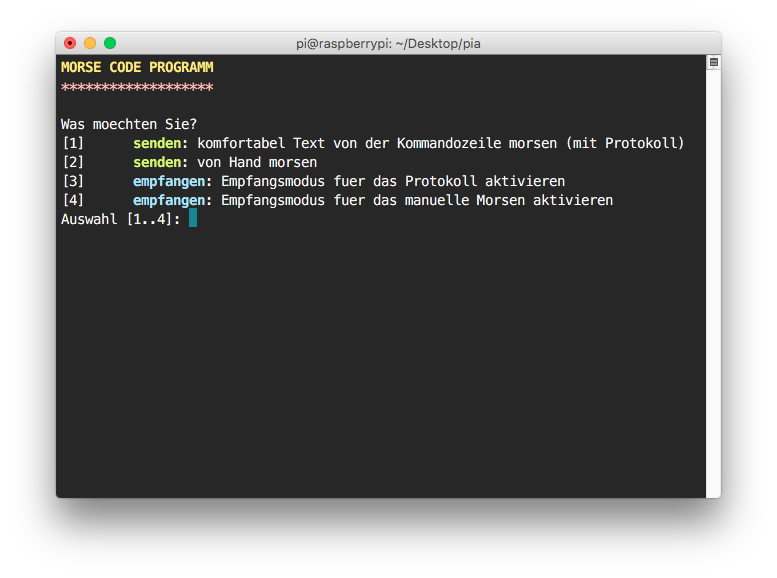
\includegraphics[width=1.0\textwidth]{sshot_1.png}
	\caption{Auf Pi A (s. Kopfzeile des Fensters) wurde das Programm gestartet.}
\end{figure}

\newpage
\begin{figure}[H]
	\centering
	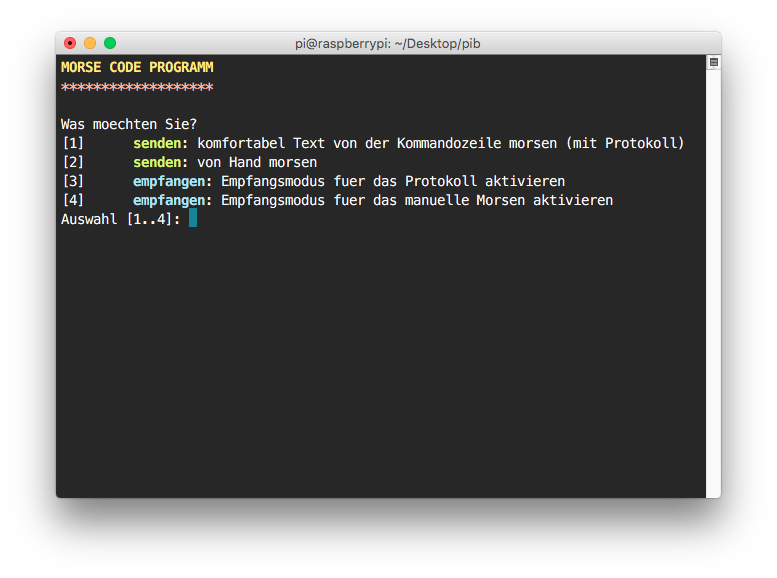
\includegraphics[width=1.0\textwidth]{sshot_2.png}
	\caption{Auf Pi B (s. Kopfzeile des Fensters) ebenfalls.}
\end{figure}

\newpage
\begin{figure}[H]
	\centering
	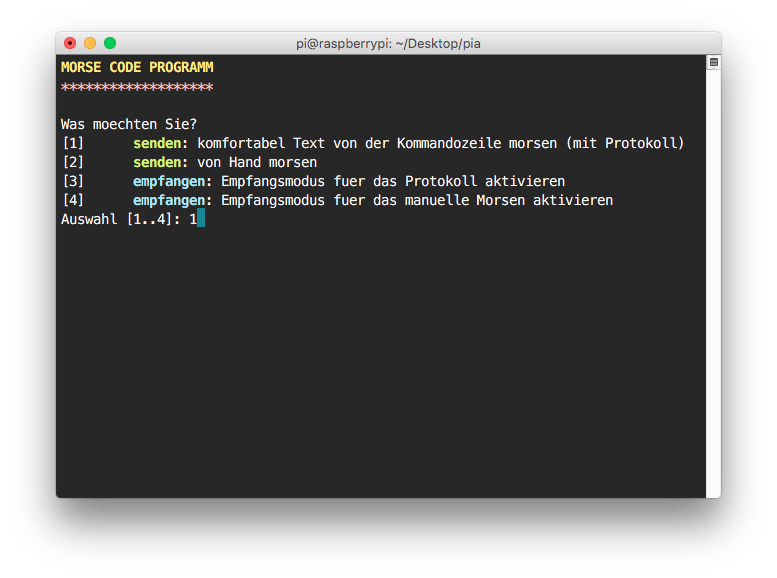
\includegraphics[width=1.0\textwidth]{sshot_3.png}
	\caption{Da ein Text mit dem Protokoll gemorst werden soll, wird auf Pi A eine \texttt{1} eingegeben.}
\end{figure}

\newpage
\begin{figure}[H]
	\centering
	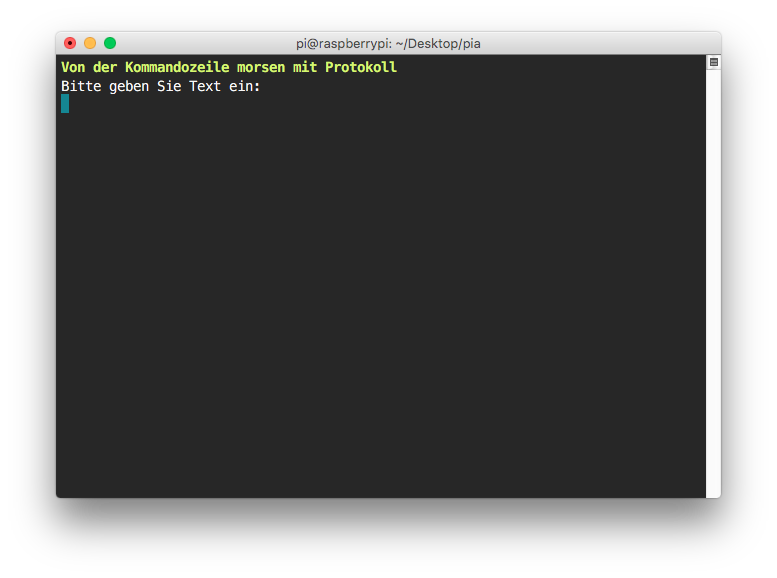
\includegraphics[width=1.0\textwidth]{sshot_4.png}
	\caption{Die Eingabeaufforderung für den Text.}
\end{figure}

\newpage
\begin{figure}[H]
	\centering
	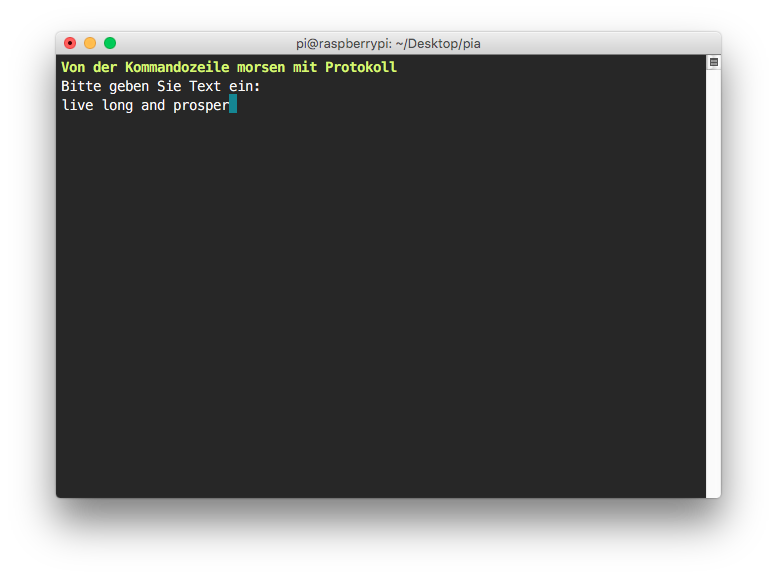
\includegraphics[width=1.0\textwidth]{sshot_5.png}
	\caption{Der Text \enquote{live long and prosper} wurde eingegeben.}
\end{figure}

\newpage
\begin{figure}[H]
	\centering
	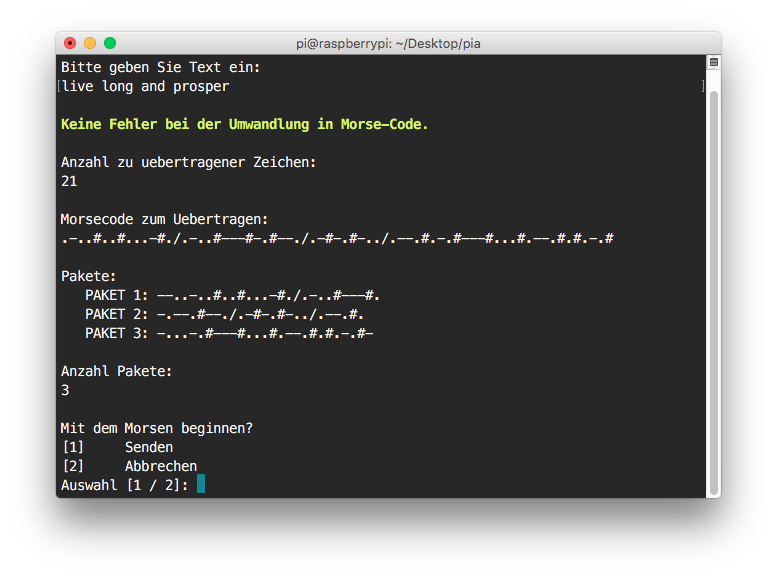
\includegraphics[width=1.0\textwidth]{sshot_6.png}
	\caption{Es hat bei der Übersetzung in Morse-Code keine Fehler gegeben. Es wurden 3 Pakete erstellt.}
\end{figure}

\newpage
\begin{figure}[H]
	\centering
	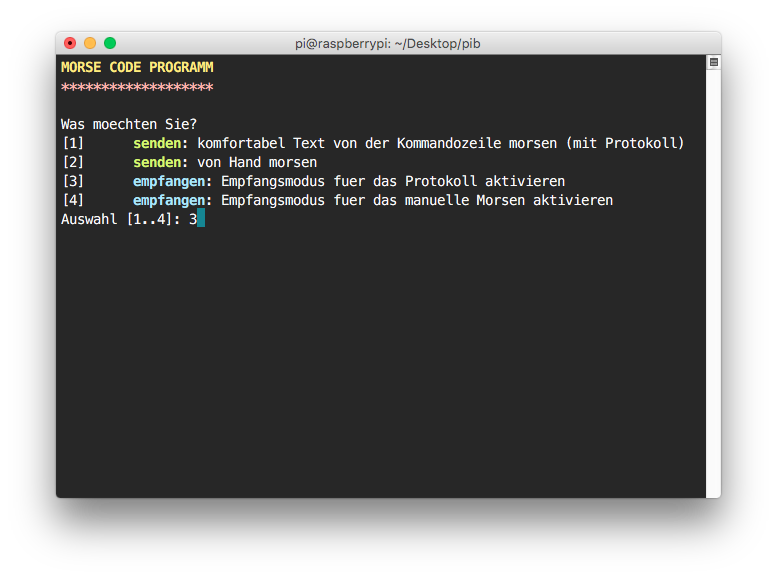
\includegraphics[width=1.0\textwidth]{sshot_7.png}
	\caption{Auf Pi B muss der Empfangsmodus ausgewählt werden.}
\end{figure}

\newpage
\begin{figure}[H]
	\centering
	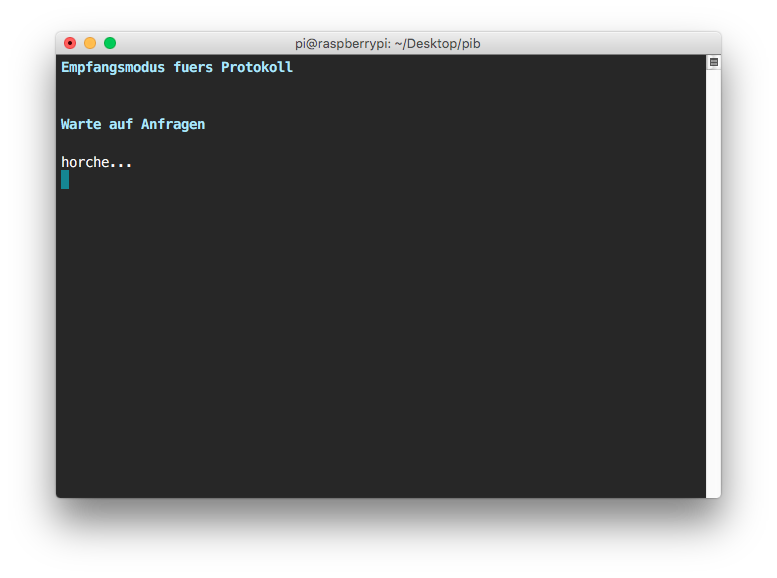
\includegraphics[width=1.0\textwidth]{sshot_9.png}
	\caption{Pi B horcht nun auf den Verbindungsaufbau...}
\end{figure}

\newpage
\begin{figure}[H]
	\centering
	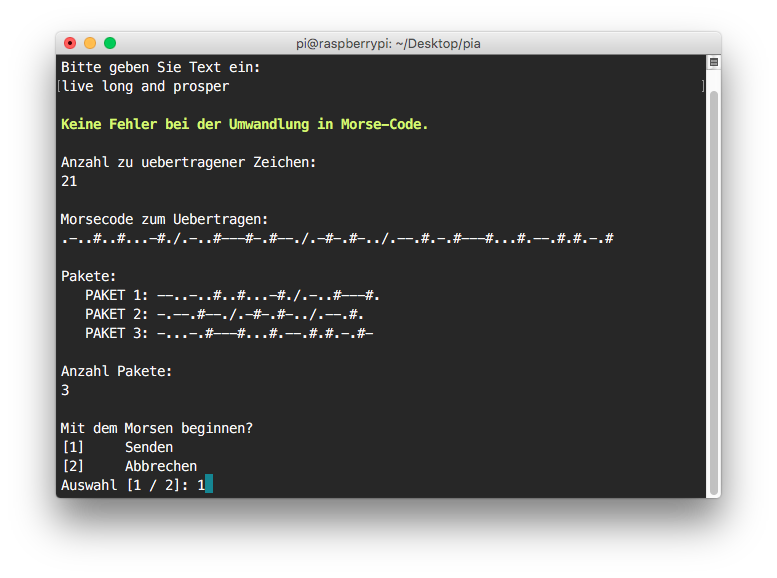
\includegraphics[width=1.0\textwidth]{sshot_8.png}
	\caption{...und auf Pi A wird das Senden durch Eingabe einer \texttt{1} gestartet.}
\end{figure}

\newpage
\begin{figure}[H]
	\centering
	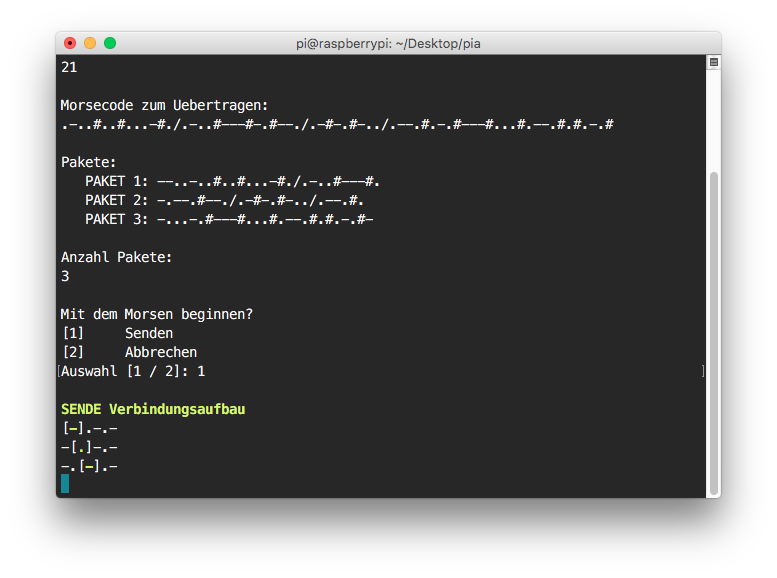
\includegraphics[width=1.0\textwidth]{sshot_10.png}
	\caption{Pi A sendet den Verbindungsaufbau...}
\end{figure}

\newpage
\begin{figure}[H]
	\centering
	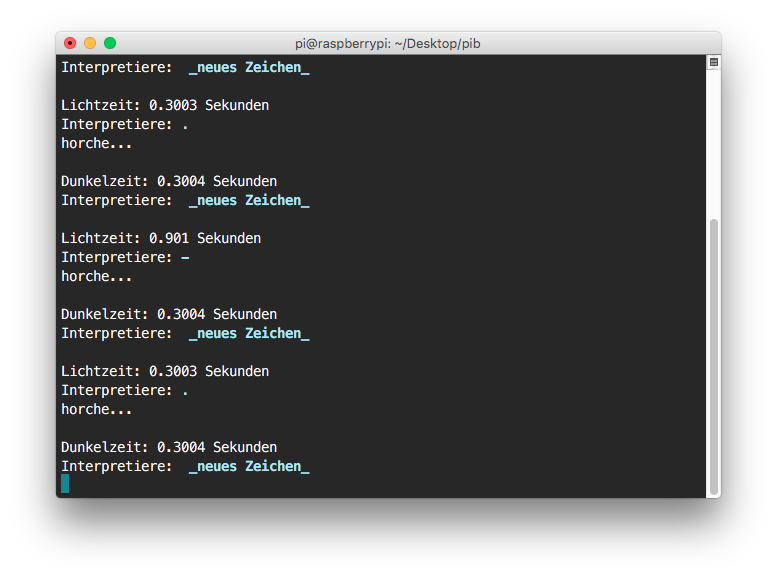
\includegraphics[width=1.0\textwidth]{sshot_11.png}
	\caption{...und Pi B empfängt ihn.}
\end{figure}

\newpage
\begin{figure}[H]
	\centering
	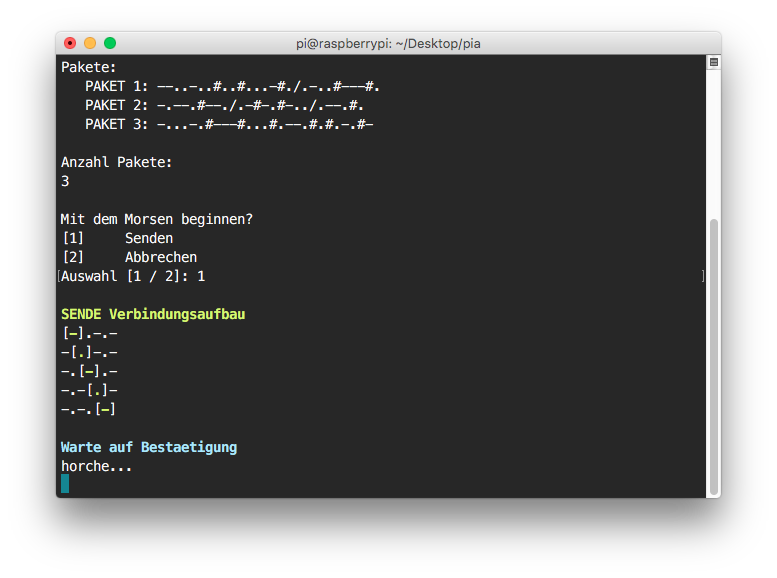
\includegraphics[width=1.0\textwidth]{sshot_12.png}
	\caption{Danach horcht Pi A auf das ACK vom Empfänger, ...}
\end{figure}

\newpage
\begin{figure}[H]
	\centering
	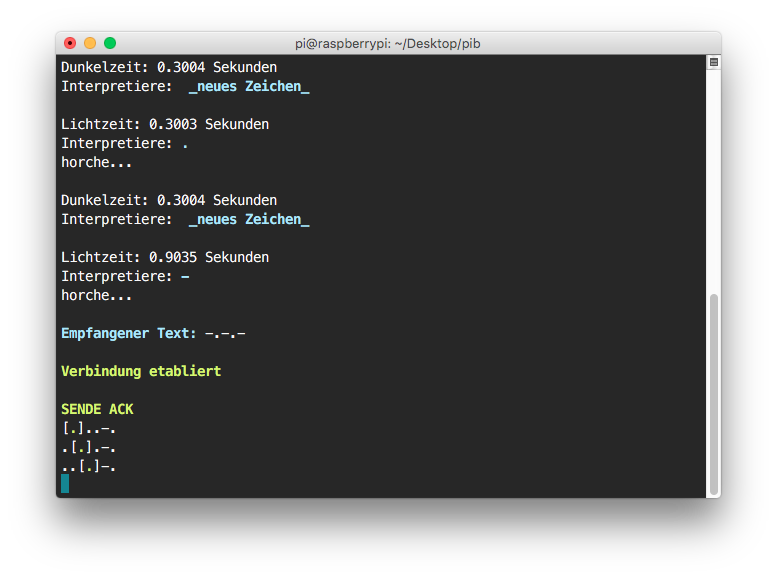
\includegraphics[width=1.0\textwidth]{sshot_13.png}
	\caption{...das von Pi B daraufhin geschickt wird.}
\end{figure}

\newpage
\begin{figure}[H]
	\centering
	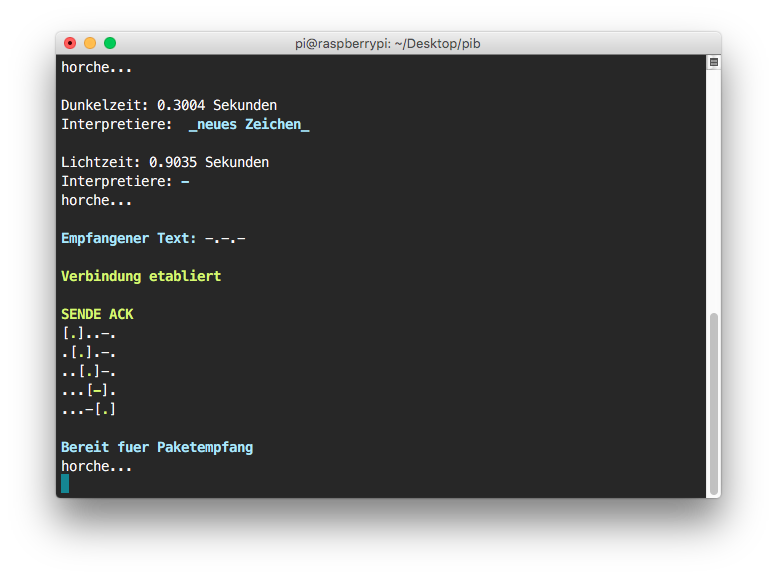
\includegraphics[width=1.0\textwidth]{sshot_14.png}
	\caption{Nach dem Senden des ACKs horcht Pi B auf das erste Paket.}
\end{figure}

\newpage
\begin{figure}[H]
	\centering
	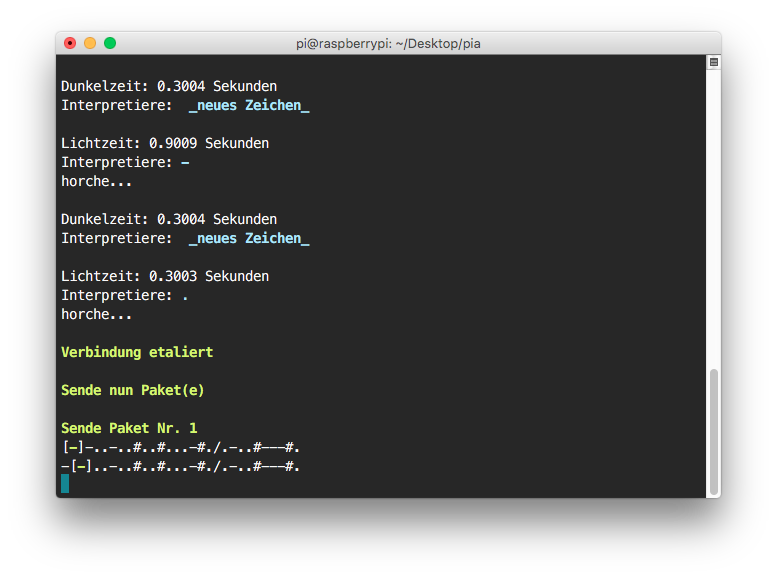
\includegraphics[width=1.0\textwidth]{sshot_15.png}
	\caption{Nach dem ACK von Pi B ist die Verbindung nun etabliert. Pi A schickt das erste Paket.}
\end{figure}

\newpage
\begin{figure}[H]
	\centering
	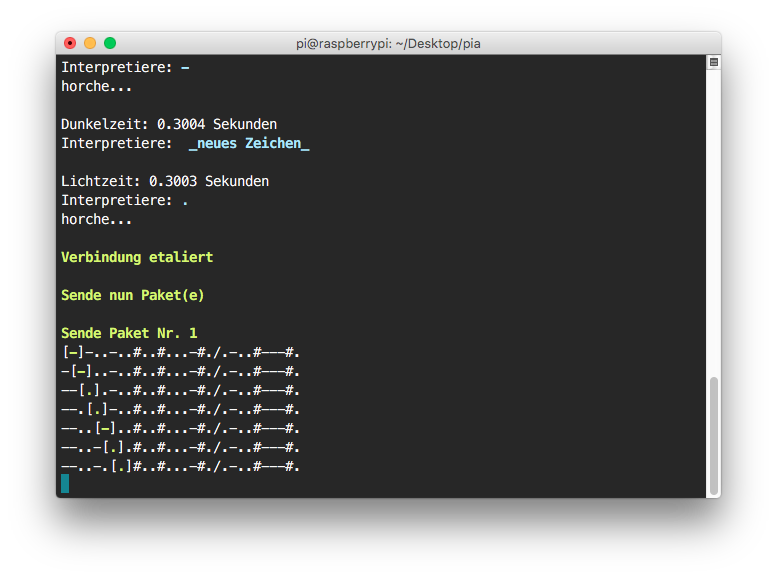
\includegraphics[width=1.0\textwidth]{sshot_16.png}
	\caption{Es wird (zufälligerweise) Paket 1 gesendet.}
\end{figure}

\newpage
\begin{figure}[H]
	\centering
	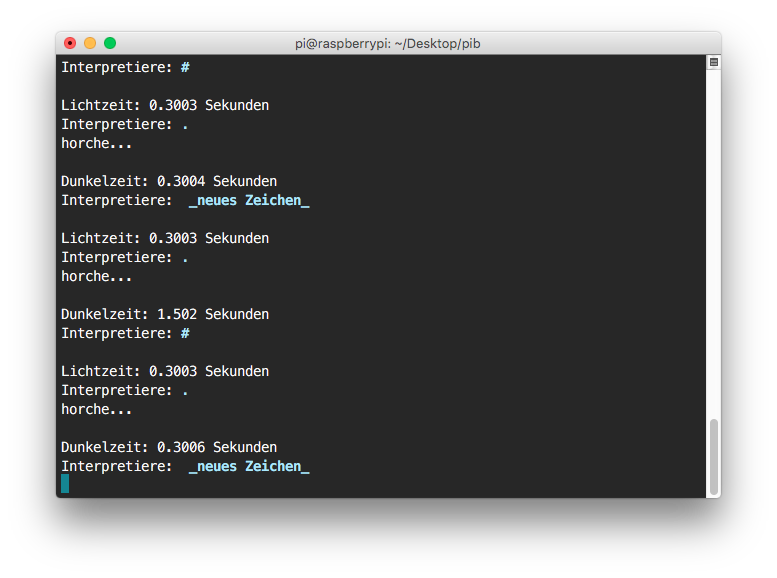
\includegraphics[width=1.0\textwidth]{sshot_17.png}
	\caption{Pi B empfängt die Lichtzeichen}
\end{figure}

\newpage
\begin{figure}[H]
	\centering
	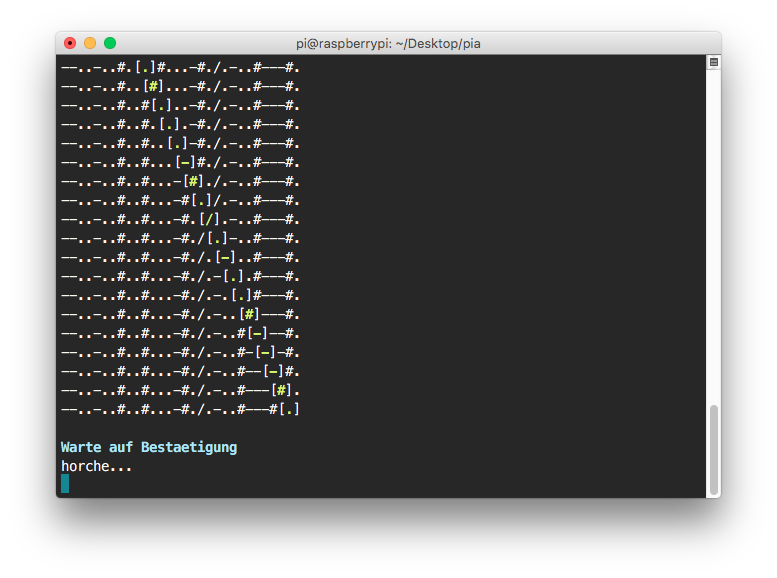
\includegraphics[width=1.0\textwidth]{sshot_21.png}
	\caption{Wenn Pi A mit dem Senden fertig ist, wartet das Programm auf eine Bestätigung.}
\end{figure}

\newpage
\begin{figure}[H]
	\centering
	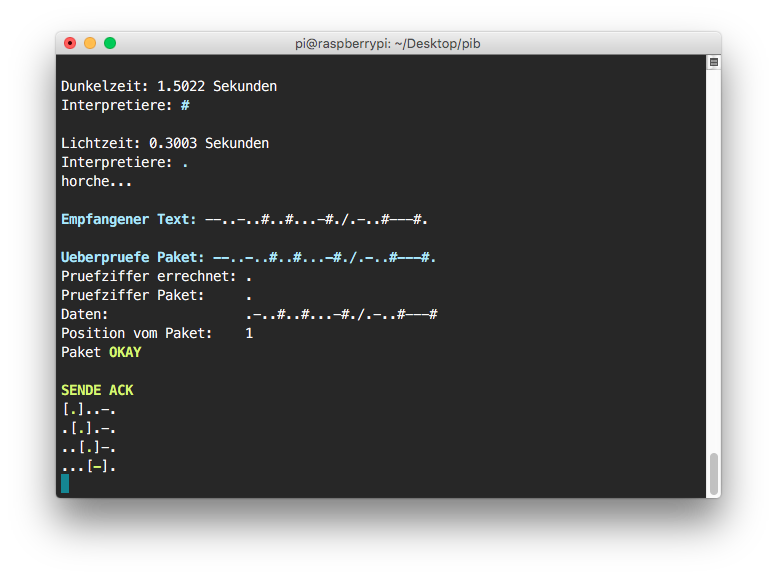
\includegraphics[width=1.0\textwidth]{sshot_22.png}
	\caption{Wenn das Paket von Pi B erfolgreich überprüft worden ist, sendet der Empfänger eine Bestätigung.}
\end{figure}

\newpage
\begin{figure}[H]
	\centering
	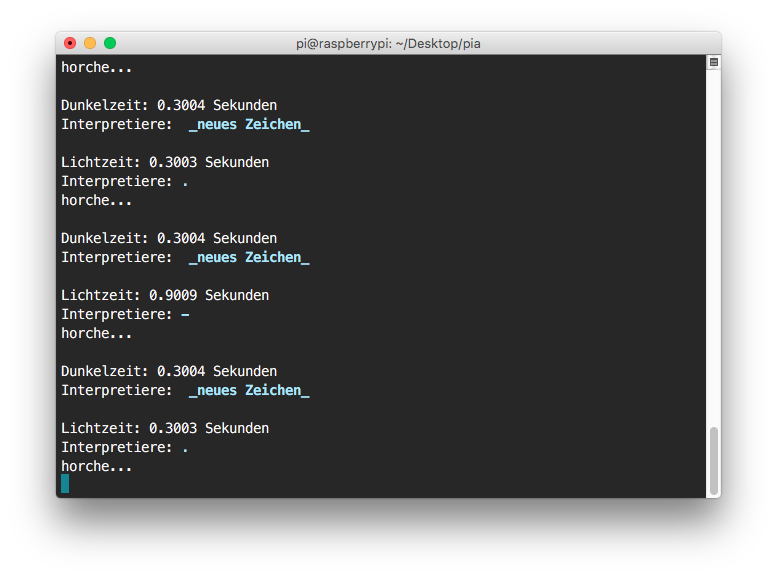
\includegraphics[width=1.0\textwidth]{sshot_23.png}
	\caption{Pi A empfängt das ACK.}
\end{figure}

\newpage
\begin{figure}[H]
	\centering
	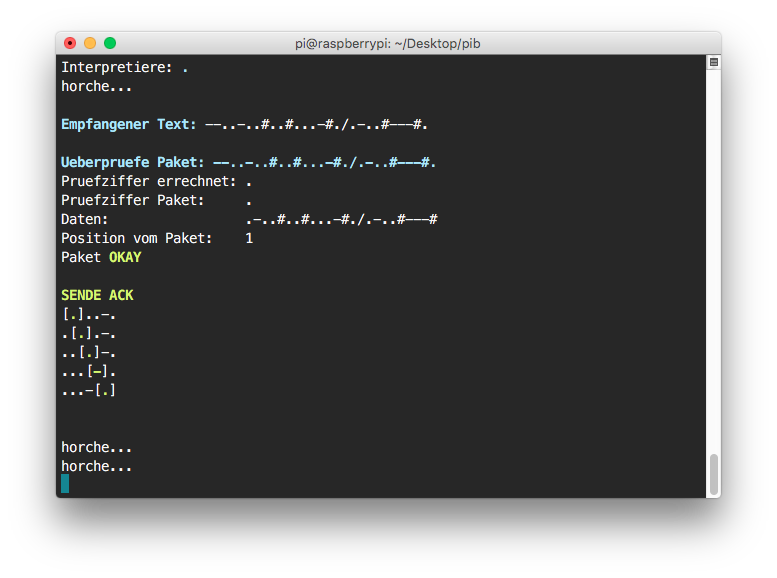
\includegraphics[width=1.0\textwidth]{sshot_24.png}
	\caption{Pi B ist inzwischen wieder im Empfangsmodus für das nächste Paket.}
\end{figure}

\newpage
\begin{figure}[H]
	\centering
	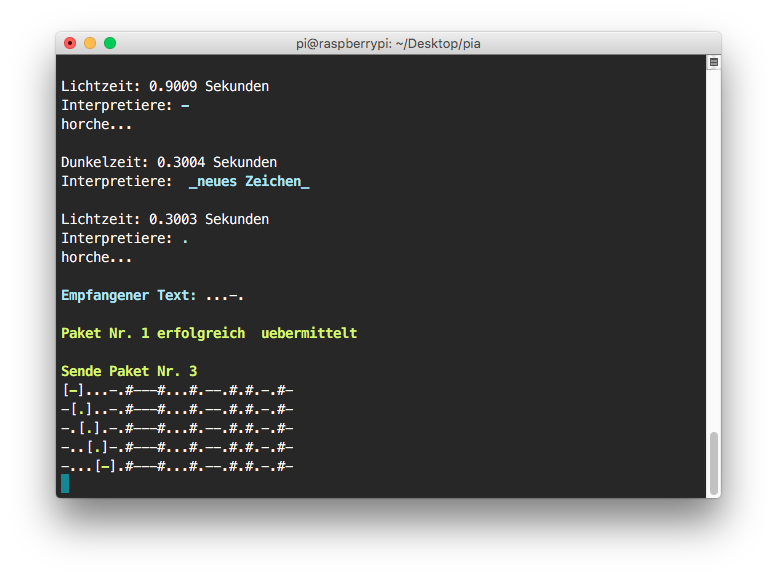
\includegraphics[width=1.0\textwidth]{sshot_25.png}
	\caption{Pi A hat das ACK empfangen und das Paket 1 aus der Liste entfernt. Nun wird Paket 3 übertragen.}
\end{figure}

\newpage
\begin{figure}[H]
	\centering
	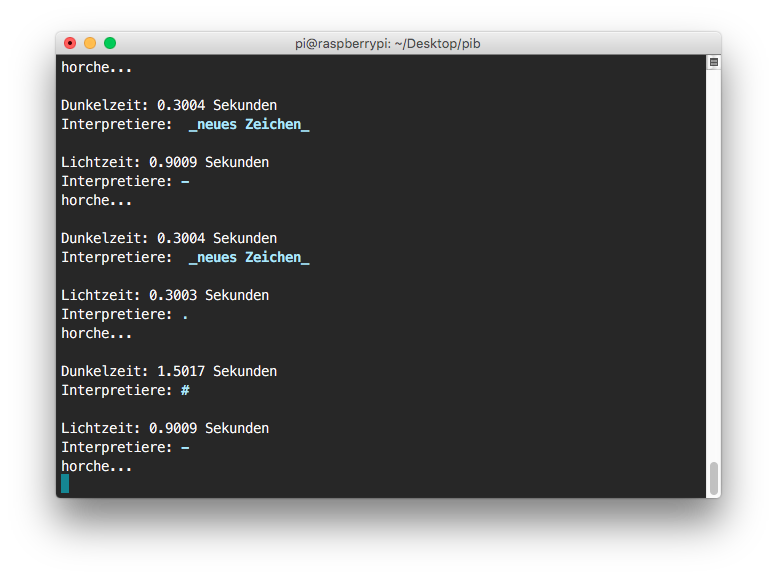
\includegraphics[width=1.0\textwidth]{sshot_26.png}
	\caption{Pi B empfängt diese Daten...}
\end{figure}

\newpage
\begin{figure}[H]
	\centering
	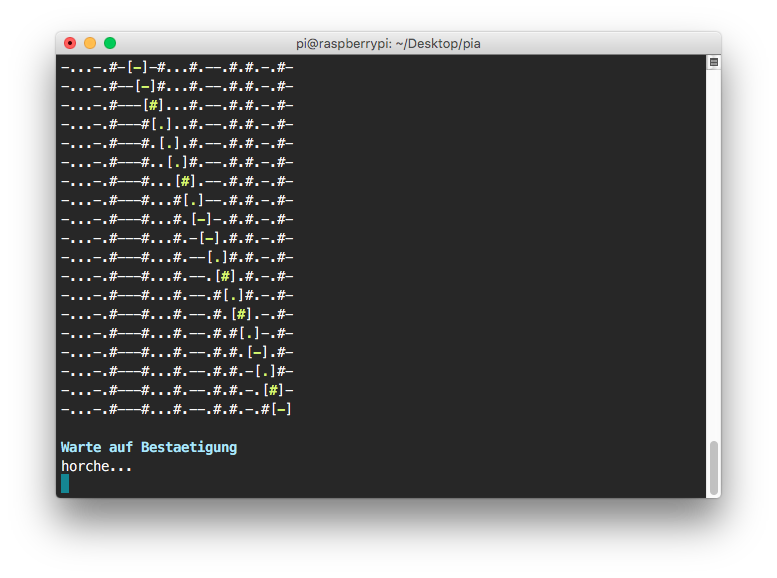
\includegraphics[width=1.0\textwidth]{sshot_31.png}
	\caption{..und Pi A geht wieder in den Empfangsmodus für die Bestätigung.}
\end{figure}

\newpage
\begin{figure}[H]
	\centering
	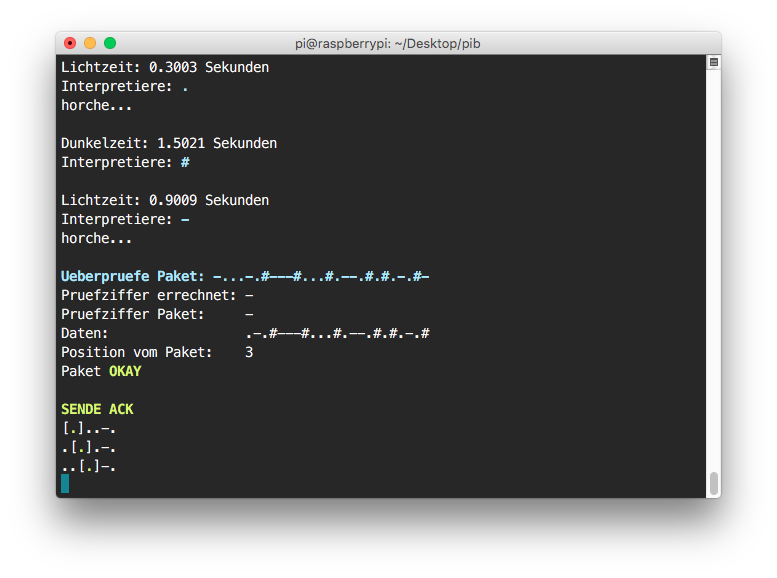
\includegraphics[width=1.0\textwidth]{sshot_32.png}
	\caption{Das Paket konnte überprüft werden und es wird eine Bestätigung geschickt.}
\end{figure}


\newpage
\begin{figure}[H]
	\centering
	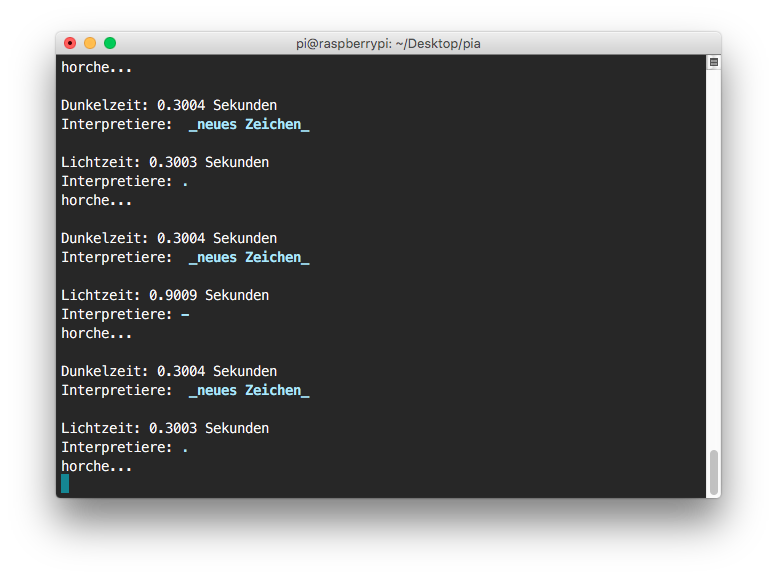
\includegraphics[width=1.0\textwidth]{sshot_33.png}
	\caption{Pi A empfängt das ACK.}
\end{figure}


\newpage
\begin{figure}[H]
	\centering
	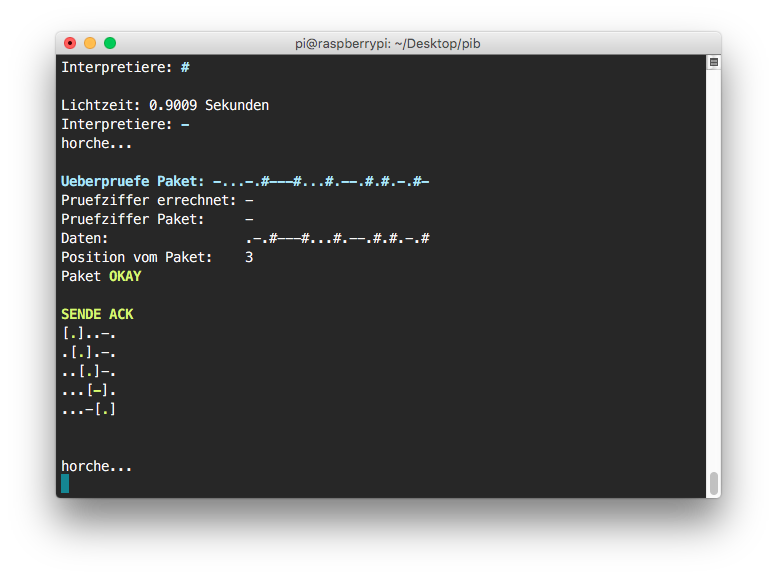
\includegraphics[width=1.0\textwidth]{sshot_34.png}
	\caption{Pi B horcht dann wieder auf das nächste Paket.}
\end{figure}




\newpage
\begin{figure}[H]
	\centering
	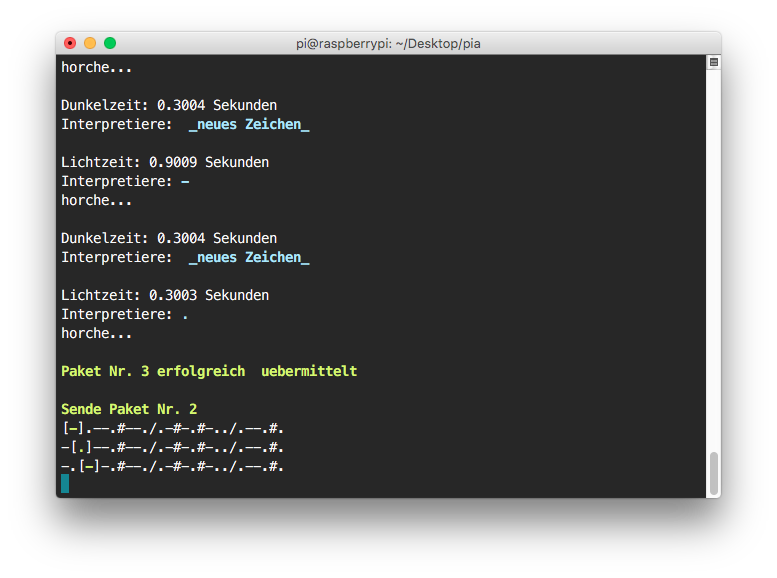
\includegraphics[width=1.0\textwidth]{sshot_35.png}
	\caption{Pi A überträgt nun das zweite Paket.}
\end{figure}

\newpage
\begin{figure}[H]
	\centering
	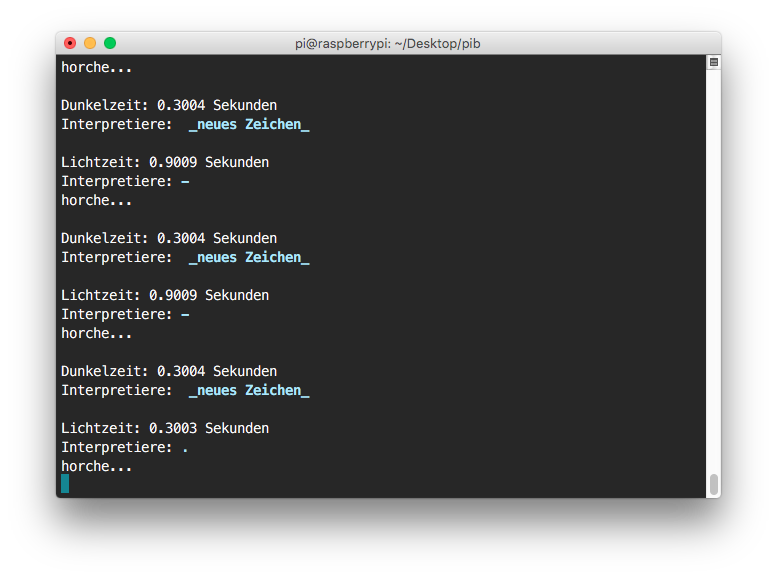
\includegraphics[width=1.0\textwidth]{sshot_36.png}
	\caption{Pi B empfängt auch das dritte Paket...}
\end{figure}

\newpage
\begin{figure}[H]
	\centering
	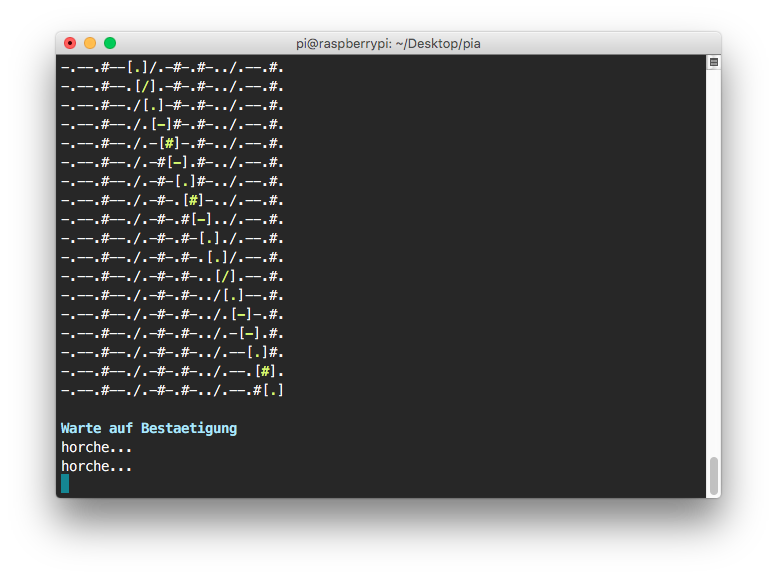
\includegraphics[width=1.0\textwidth]{sshot_41.png}
	\caption{...und horcht danach auf die Bestätigung des Pakets.}
\end{figure}

\newpage
\begin{figure}[H]
	\centering
	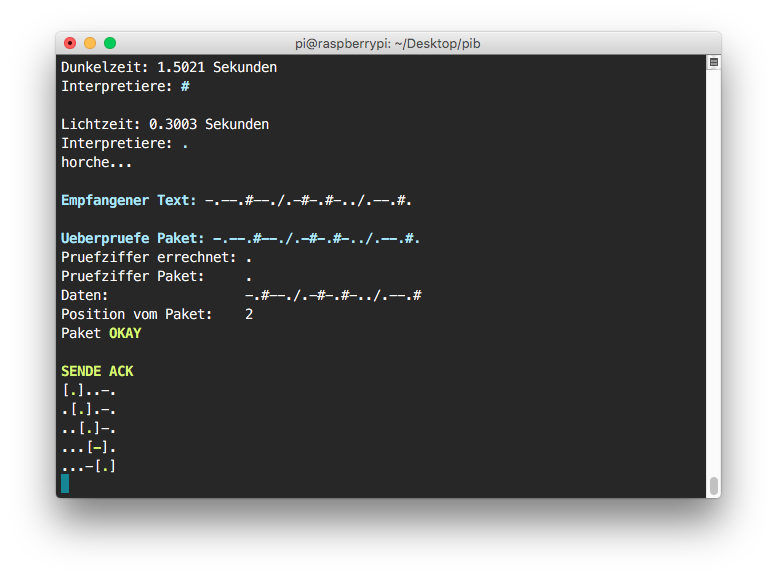
\includegraphics[width=1.0\textwidth]{sshot_42.png}
	\caption{Diese wird von Pi B geschickt, da das Paket erfolgreich überprüft werden konnte.}
\end{figure}

\newpage
\begin{figure}[H]
	\centering
	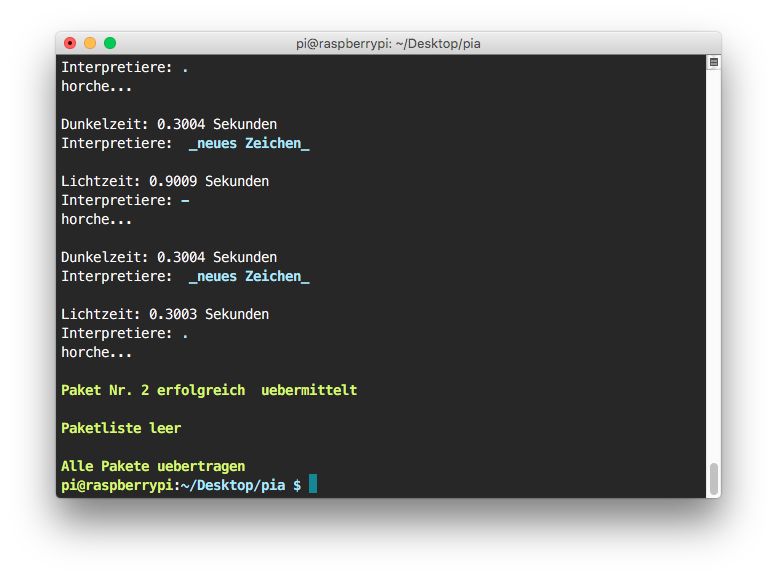
\includegraphics[width=1.0\textwidth]{sshot_43.png}
	\caption{Damit sind alle Pakete von Pi A übertragen. Das Programm beendet sich.}
\end{figure}

\newpage
\begin{figure}[H]
	\centering
	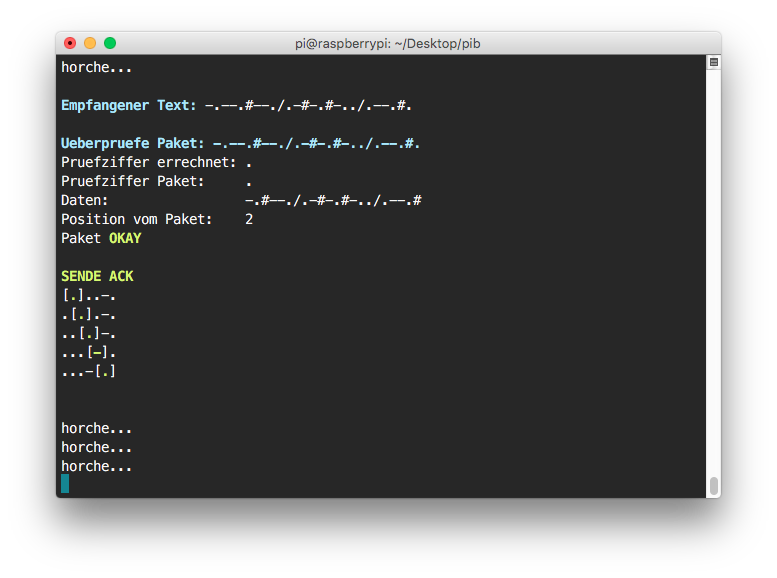
\includegraphics[width=1.0\textwidth]{sshot_45.png}
	\caption{Pi B horcht erstmal auf weitere Pakete.}
\end{figure}

\newpage
\begin{figure}[H]
	\centering
	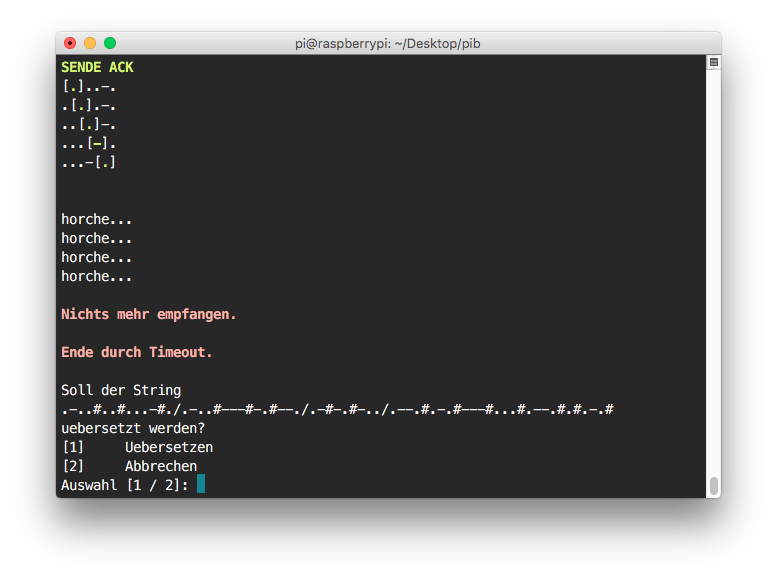
\includegraphics[width=1.0\textwidth]{sshot_46.png}
	\caption{Pi B kann nicht wissen, ob alle Pakete empfangen wurden. Da nichts mehr empfangen wurde, bricht das Programm ab (Timeout), und bietet die Möglichkeit an, den empfangenen Morse-Code-String zu übersetzen.}
\end{figure}

\newpage
\begin{figure}[H]
	\centering
	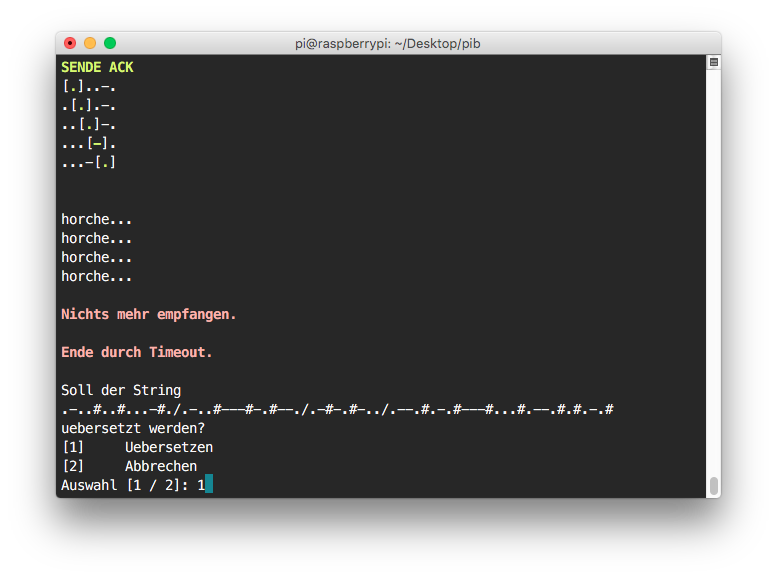
\includegraphics[width=1.0\textwidth]{sshot_48.png}
	\caption{Durch Eingabe von einer \texttt{1} kann der String übersetzt werden.}
\end{figure}

\newpage
\begin{figure}[H]
	\centering
	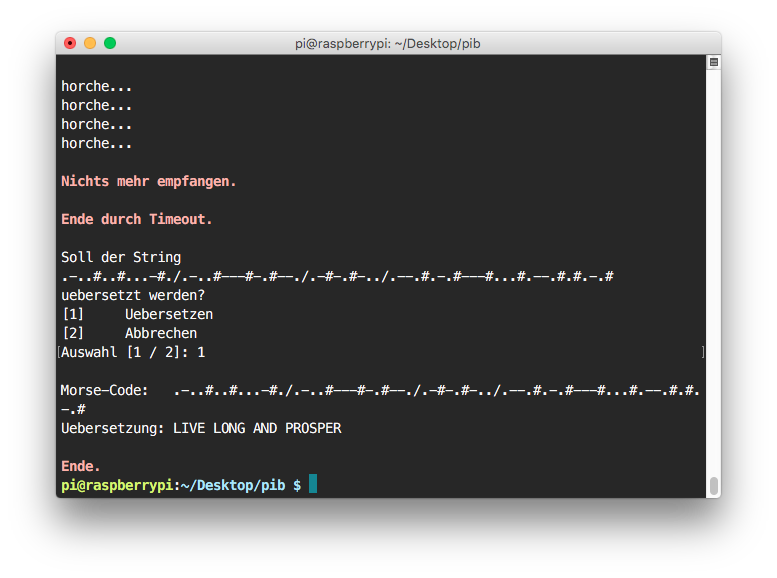
\includegraphics[width=1.0\textwidth]{sshot_49.png}
	\caption{Die Übersetzung wird angezeigt und das Programm beendet sich.}
\end{figure}

\end{document}